%%%%%%%%%%%%%%%%%%%%%%%%%%%%%%%%%%%%%%%%%%%%%%%%%%%%%%%%%%%%%%%
%
% Welcome to Overleaf --- just edit your LaTeX on the left,
% and we'll compile it for you on the right. If you give 
% someone the link to this page, they can edit at the same
% time. See the help menu above for more info. Enjoy!
%
%%%%%%%%%%%%%%%%%%%%%%%%%%%%%%%%%%%%%%%%%%%%%%%%%%%%%%%%%%%%%%%

%  My thanks to Dana Ernst of Northern Arizona University for sharing 
%    his template with me. This is largely his work.
% --------------------------------------------------------------
% This is all preamble stuff that you don't have to worry about.
% Head down to where it says "Start here"
% --------------------------------------------------------------
 
\documentclass[12pt]{article}
 
\usepackage[margin=1in]{geometry} 
\usepackage{amsmath,amsthm,amssymb}
\usepackage{graphicx}
 
\newenvironment{theorem}[2][Theorem]{\begin{trivlist}
\item[\hskip \labelsep {\bfseries #1}\hskip \labelsep {\bfseries #2.}]}{\end{trivlist}}
\newenvironment{lemma}[2][Lemma]{\begin{trivlist}
\item[\hskip \labelsep {\bfseries #1}\hskip \labelsep {\bfseries #2.}]}{\end{trivlist}}
\newenvironment{conjecture}[2][Conjecture]{\begin{trivlist}
\item[\hskip \labelsep {\bfseries #1}\hskip \labelsep {\bfseries #2.}]}{\end{trivlist}}
\newenvironment{question}[2][Question]{\begin{trivlist}
\item[\hskip \labelsep {\bfseries #1}\hskip \labelsep {\bfseries #2.}]}{\end{trivlist}}
\newenvironment{corollary}[2][Corollary]{\begin{trivlist}
\item[\hskip \labelsep {\bfseries #1}\hskip \labelsep {\bfseries #2.}]}{\end{trivlist}}
\newenvironment{definition}[2][Definition]{\begin{trivlist}
\item[\hskip \labelsep {\bfseries #1}\hskip \labelsep {\bfseries #2.}]}{\end{trivlist}}

\begin{document}
 
% --------------------------------------------------------------
%                         Start here
% --------------------------------------------------------------
 
\title{Class Journal Template} % replace with an appropriate title, choose something shortish & descriptive
\author{Your Name} % replace with your name, multiple authors go in alphabetical order by last name
 
\maketitle

{%
\centering
\textit{Communicated by: Ms. Prooffixer} % replace the name with the name of your referee(s)
\par
}
\hrule
\vspace{.2in}


If you feel it is appropriate to include any comments as an introduction, it should go here.

\begin{lemma}{x.yz} %You can use theorem, lemma, conjecture, question, corollary, definition
xercise, problem, or question here.  Modify x.yz to be whatever number you are proving
Delete this text and write your statement here. Change the x.yz to use a numbering consistent with our class scheme.
\end{lemma}
 
\begin{proof}  
Blah, blah, blah. Delete this and write your proof here.
\end{proof}
 
\begin{theorem}{x.yz}
this is a theorem
\end{theorem}
 
\begin{proof}
Blah, blah, blah.  I'm so smart. This is another proof. Here is how you include a figure:

\begin{figure}[ht]
\centering
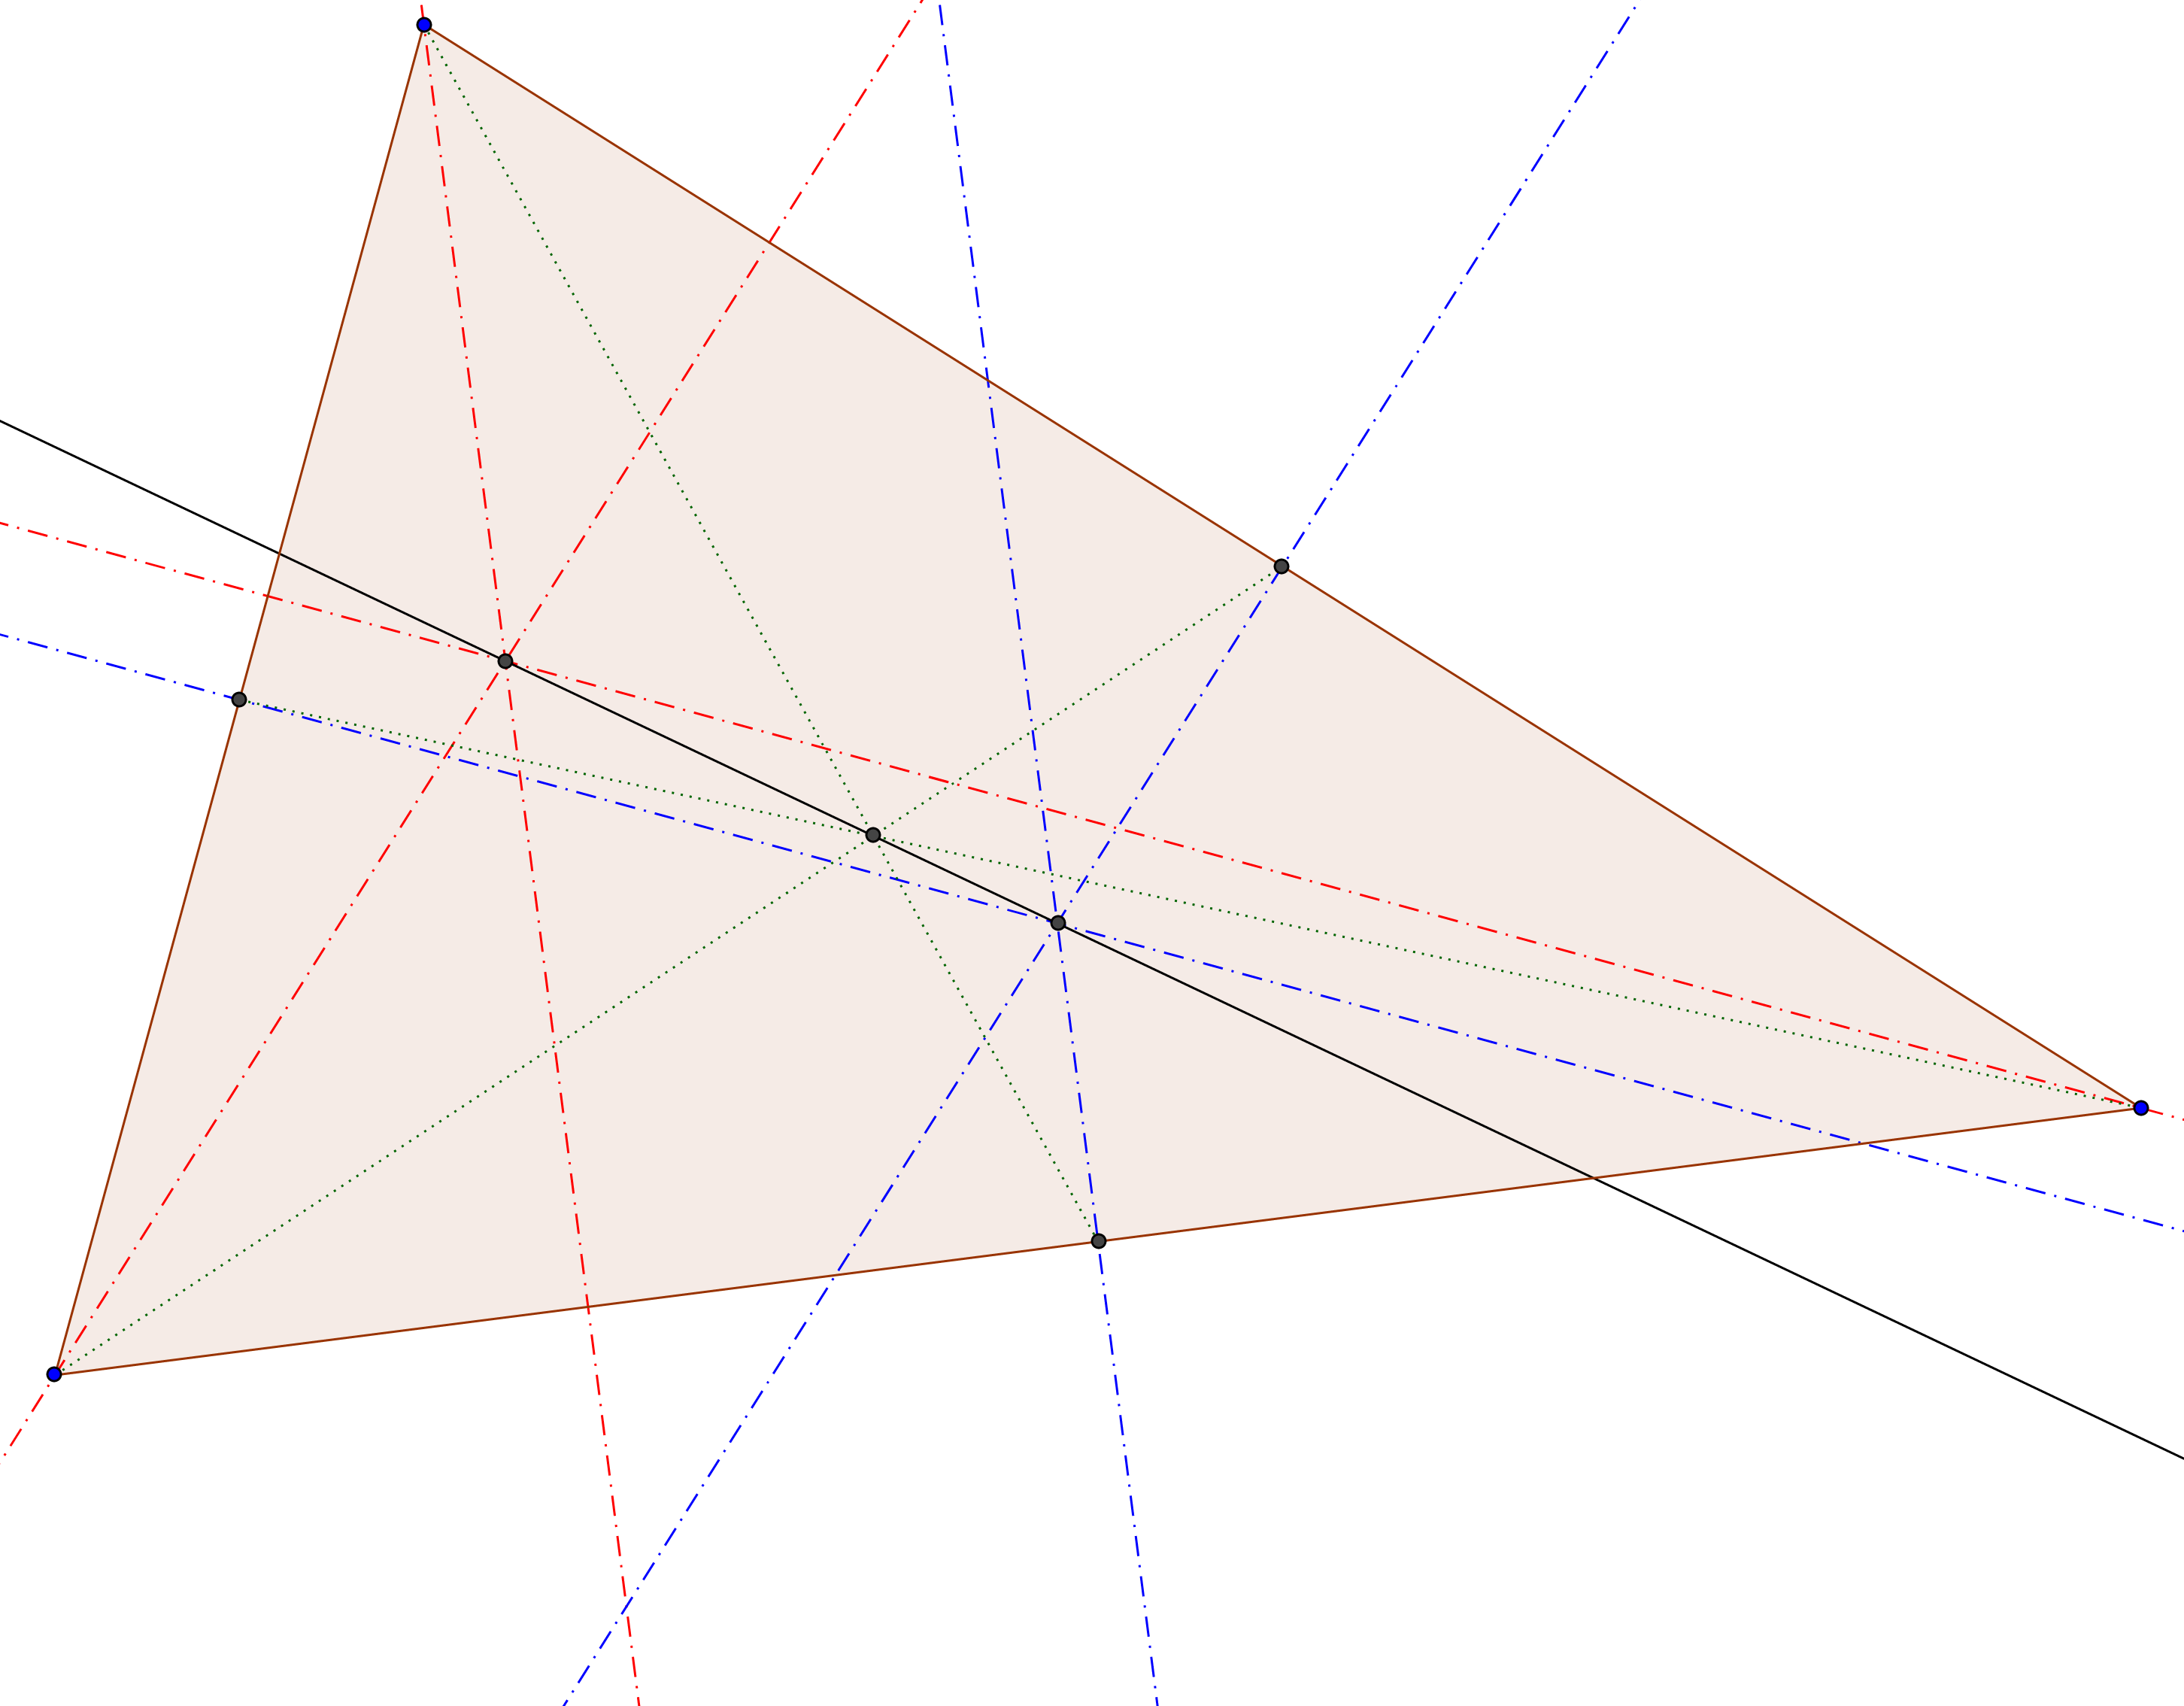
\includegraphics[width=.5\textwidth]{TEG_cover.png}
\caption{This is a picture of math.}
\end{figure}


After your figure you can have more text. It is possible to change the way your figure is placed and sized. Play around with the parameters to see what happens.

By the way, that figure was made with GeoGebra, using its ``export" feature to download the image I wanted. It works well to use ".png" files. Then I uploaded that into overleaf.com using the ``files -- upload figures \dots'' menu item.
\end{proof}
 
% --------------------------------------------------------------
%     You don't have to mess with anything below this line.
% --------------------------------------------------------------
 
\end{document}